
\begin{comment}
\subsection{Supply versus Demand}
The treatment effects that we observe are the product of changes in the identity of who becomes a political leader, as well as, potential changes in how citizens engage with the elected political class, say by demanding that they control deforestation. While both changes are consistent with an improved representation story, we can make some progress in judging the likelihood of the two stories. If demand effects are salient, we should see larger treatment effects in areas that have an ex-ante ST plurality because the preferences of the electorate around renewable resources are most likely to get represented when politicians are likely to be selected from their communities. To test this mechanism, we first define ST Plurality as ST Population Share - Non-ST Population Share, which is distributed on $[-1, 1]$ (villages with no ST have -1 ST Majority, while villages that are exclusively ST have 1). We then interact the treatment indicator in \ref{styfe} with bins of the ST Plurality variable to flexibly capture the treatment effect as a function of ST majority. This allows the treatment effect to vary non-linearly by bin (as suggested by \parencite{hainmueller2019much}) as opposed to imposing a strong linear form using a linear interaction term. 

We fail to rule out the null of uniform treatment effects as a function of ST composition, as reflected in ~\ref{fig:intflex_stmaj}. Interpreting interior values is somewhat challenging given the distribution of ST majorities, which is highly bimodal: they are either a negligible share of the electorate or constitute a plurality, see \ref{fig:st_share_dist}), and as a result, coefficients for intermediate values are estimated imprecisely. Furthermore, since one of the key criteria for PESA designation was ST population share, treatment overlap is weak over the distribution of the ST majority share. Overall, we interpret this as suggestive evidence that demand effects are not the primary divers of the treatment effects we observe.

% \begin{centering}
% \begin{table}[!htbp] \centering
%   \caption{Regressions with ST Plurality Interaction}
%   \label{table:regres}
%   \input{Output/plurality_test_regs.tex}
% \end{table}
% \end{centering}


\begin{figure}[htbp!]
\begin{center}
\begin{minipage}{1 \linewidth}
  \caption{\textbf{Treatment effects on Annual Deforestation by ST Plurality}\label{fig:intflex_stmaj}	}
\centerline{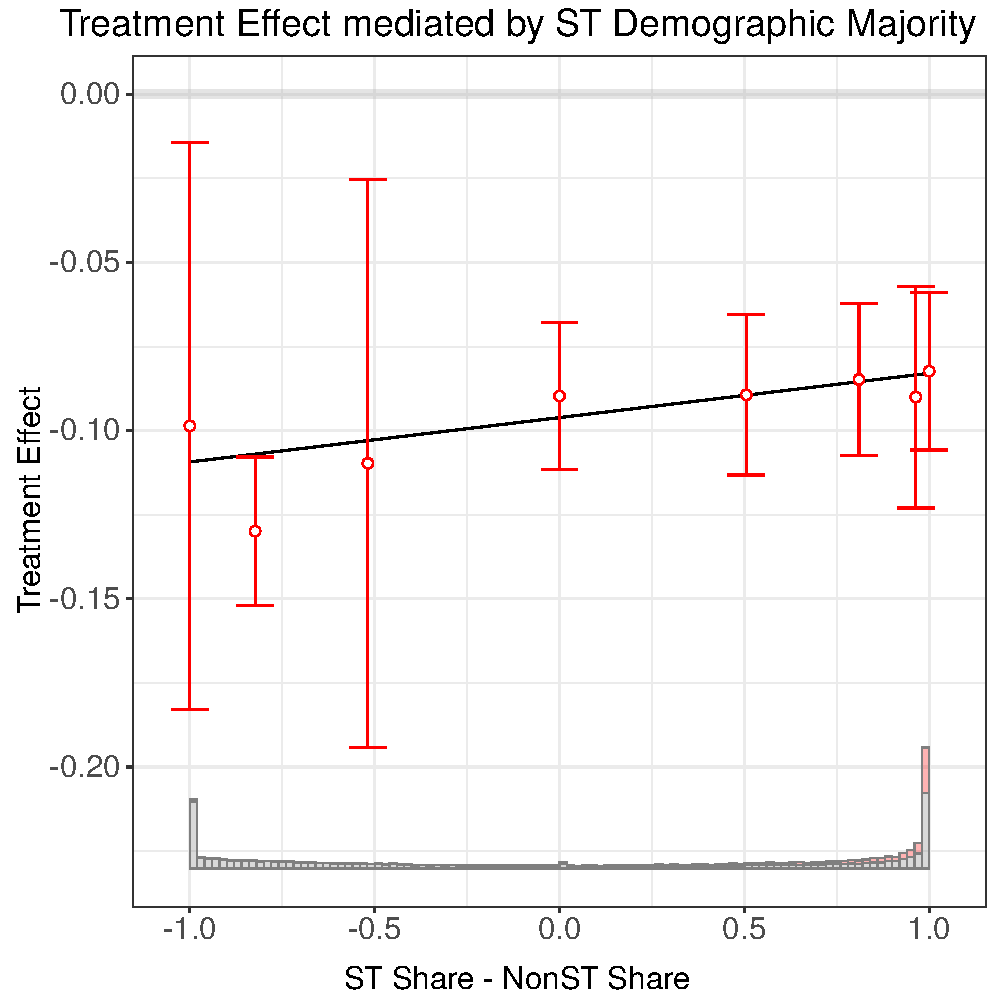
\includegraphics[width=3 in,angle=0]{Output/Interflex_stmaj.pdf}}
\smallskip
\scriptsize
\emph{Notes}: As with Figure ~\ref{fig:intflex_stmaj}, the Figure reports coefficient estimates from a binned saturated regression using \texttt{interflex}, using the population share gap between ST and Non-ST groups as a moderator, which serves as a measure for the STs electoral plurality.
\end{minipage}
\end{center}
\end{figure}

\end{comment}

\pagebreak
